\documentclass[a4paper]{article}

\usepackage[utf8]{inputenc}
\usepackage[spanish]{babel}
\usepackage[margin=2cm, top=2cm, includefoot]{geometry}%--para definir espacio de márgenes
\usepackage{graphicx}%--para insertar imágenes
\usepackage{fancyhdr}%--para el estilo con barra arriba de las páginas
\usepackage[table,xcdraw]{xcolor}%--para la detección de colores
\usepackage[hidelinks]{hyperref}%--para hipervínculos
\usepackage{parskip}%--para evitar tabulación de inicio de párrafo
\usepackage{booktabs}%--
\usepackage{multirow, array}
\usepackage{ragged2e}
\usepackage{float}

%definiendo color
\definecolor{rojoOscuro}{HTML}{A20303}
%---definiendo estilo del informe
\setlength{\headheight}{56.10185pt}
\pagestyle{fancy}
\fancyhf{}
\lhead{\hspace{0.1cm} 
\includegraphics[height=1.55cm]{../imagenes/CiberSecFIIS.png}}\rhead{
\includegraphics[height=1.5cm]{../imagenes/uni_logo.png} \hspace{0.1cm}}

%---Cambios
\renewcommand{\headrulewidth}{3pt}%--grosor de la linea superior
\renewcommand{\headrule}{\hbox to\headwidth{\color{rojoOscuro}\leaders\hrule height \headrulewidth\hfill}}%--definir la linea base superior
\renewcommand{\arraystretch}{2}%--espaciado de las tablas
%---Inicio de informe

\begin{document}
    \begin{titlepage}
    \centering
        {\large \textbf{UNIVERSIDAD NACIONAL DE INGENIERÍA}} \par \vspace{0.3cm}
        {\large \textbf{FACULTAD DE INGENIERÍA INDUSTRIAL Y DE SISTEMAS}} \par \vspace{1.125cm}
        
\includegraphics[width=0.7\textwidth]{imagenes/CiberSecFIIS.png} \par \vspace{1.125cm}
        {\LARGE \textbf{Segunda Evaluación de Penetración de Seguridad}}\par \vspace{1cm}
        {\Large \textbf{Elaborado por:}} \par \vspace{1cm}
        \vfill
        {\large \textbf{Carolina Aliaga}} \par \vspace{0.8cm}
        {\large \textbf{Elian Paucar}} \par \vspace{3.55cm}
        \vfill
        {\textbf{Lima, 2021}}
\end{titlepage}

%-----------------------------------------------------------
    \clearpage
        \tableofcontents
    \clearpage
%------------------------------------------------------------
    \listoffigures
    \clearpage
%------------------------------------------------
    %----Para el inicio de numeración a partir de aquí---
    \cfoot{\thepage}
    \setcounter{page}{1}
 %--------Resumen ejecutivo------------
    \addcontentsline{toc}{section}{Resumen Ejecutivo} %--Para que sección sin numeración aparezca en el índice
    \begin{center}
        \section*{Resumen Ejecutivo}
    \end{center}
    \vspace{0.1cm}

%-------------------------------------------------
    \clearpage
    \section{Objetivo}
        \large{El objetivo de la presente evaluación de penetración de seguridad es encontrar vulnerabilidades y hacer una evaluación de criticidad de estas con el fin de que el negocio no se vea afectado por algún ataque malicioso que pueda afectar la calidad de sus servicios y su imagen.}
        \par
    \section{Alcance}
        \large{El alcance de esta evaluación se limita a las pruebas en los computadores de la plataforma Hack The Box con las siguientes direcciones IP:}
        \par
        \begin{table}[h]
            \centering
                \begin{tabular}{|c|c|c|c|c|} \hline
                    Identificador & Nombre de host & Dirección IP & Sistema Operativo & Dificultad \\ \hline
                    
                \end{tabular}
                \caption{Datos sobre las máquinas}
        \end{table}
        \par
    \section{Detalle de Hallazgos}
        \large{Los hallazgos encontrados en la evaluación de penetración de seguridad fueron los siguientes:}
        \par
        \large{Se encontraron 4 vulnerabilidades entre las 3 máquinas.}
        \par
        \begin{table}[H]
            \centering
                \begin{tabular}{|c|c|c|c|c|c|c|}\hline
                    Identificador & CVE & Tipo de vulnerabilidad & CVSSv2 & Jarvis & Time & Forest \\ \hline
                    
                \end{tabular}
                \caption{Vulnerabilidades encontradas}
        \end{table}
        \par
        

%------Pruebas de penetracion----------
    \clearpage
    \subsection{HTB04 - Friendzone}

    \subsubsection{Escaneo}
        \large{Como primera etapa de la Prueba de Penetración realizamos un escaneo de puertos abiertos en la máquina víctima con la herramienta "Nmap", donde se encuentran siete de ellos.}
        \par
        \begin{figure}[H]
            \centering
            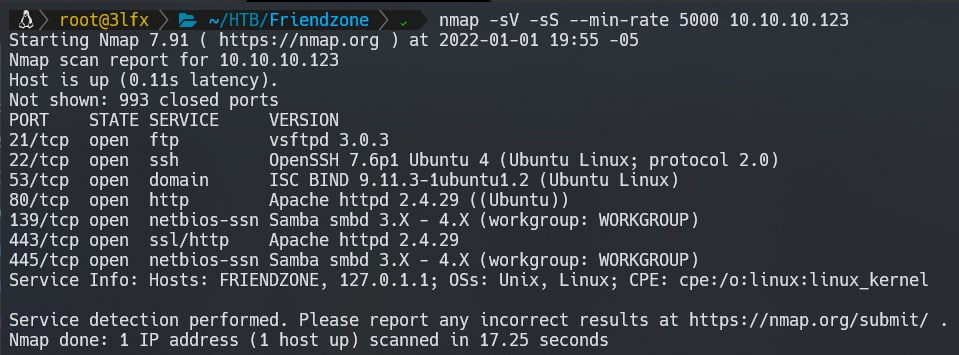
\includegraphics[width=0.99\textwidth]{informe4/imagenes/friendzone/01_escaneo.png}
            \caption{Escaneo de puertos Friendzone} 
        \end{figure}  

    \subsubsection{Análisis de Vulnerabilidades}
        \large{Se intenta acceder a la máquina mediante el puerto 'ftp', pero no se consigue el acceso.}
        \par
        \begin{figure}[H]
            \centering
            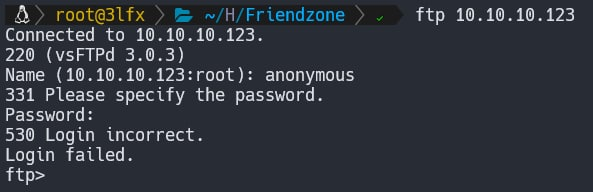
\includegraphics[width=0.99\textwidth]{informe4/imagenes/friendzone/02_ftp.png}
            \caption{Puerto ftp en Friendzone} 
        \end{figure}
        
        \large{Luego probamos con el puerto 'netbios ssn', usando la herramienta 'smbmap'.}
        \par
        \begin{figure}[H]
            \centering
            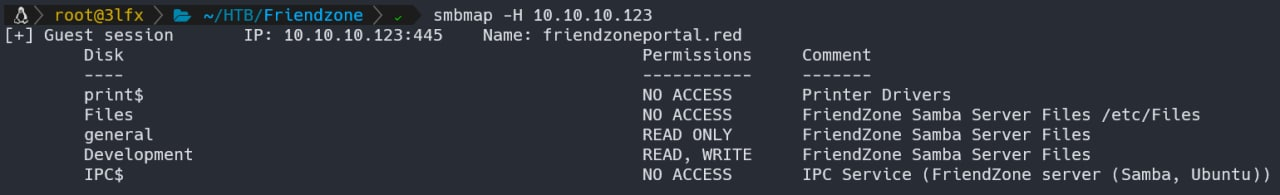
\includegraphics[width=0.99\textwidth]{informe4/imagenes/friendzone/03_smbmap.png}
            \caption{Hallazgo de la herramienta smbmap en Friendzone} 
        \end{figure}

        \large{Identificamos dos carpeta a las que se tiene acceso, una llamada genarl con acceso solo para leer y otra con nombre Development con accesos para leer y escribir. Revisamos la carpeta general.}
        \par
        \begin{figure}[H]
            \centering
            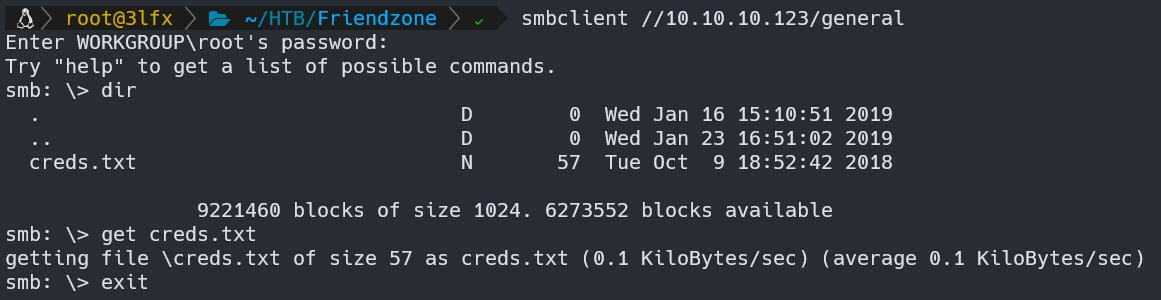
\includegraphics[width=0.99\textwidth]{informe4/imagenes/friendzone/04_smb_creds.png}
            \caption{Carpeta general en Friendzone} 
        \end{figure}

        \large{Dentro de la carpeta general encontramos una archivo '.txt' con el nombre creds, el cual parece una abreviacion de credenciales, por lo cual revisamos el archivo y al hacerlo encontramos las credenciales de admin.}
        \par
        \begin{figure}[H]
            \centering
            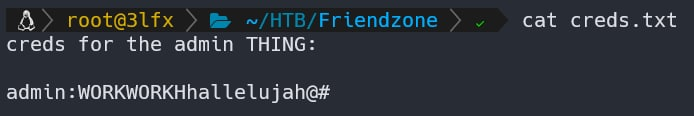
\includegraphics[width=0.99\textwidth]{informe4/imagenes/friendzone/05_cred_friendzone.png}
            \caption{Archivo creds.txt en Friendzone} 
        \end{figure}




    \subsubsection{Explotación}

    \subsubsection{Escalamiento de Privilegios}
        \large{Ya dentro de la maquina buscamos acceder a las carpetas a la que el usuario tiene acceso.}
        \par
        \begin{figure}[H]
            \centering
            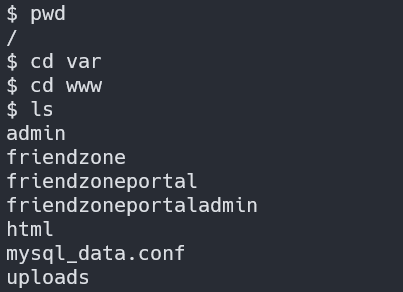
\includegraphics[width=0.99\textwidth]{informe4/imagenes/friendzone/20_enum_varwww.png}
            \caption{Enum varwww en Friendzone} 
        \end{figure}

        \large{Leemos el contenido del archivo 'mysql data.conf'.}
        \par
        \begin{figure}[H]
            \centering
            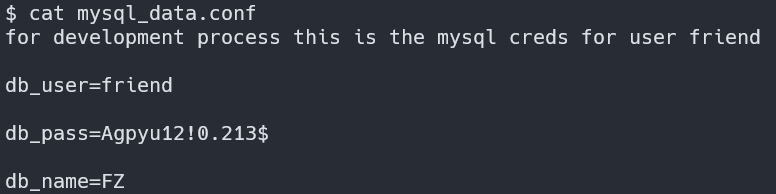
\includegraphics[width=0.99\textwidth]{informe4/imagenes/friendzone/21_password_friend.png}
            \caption{Archivo mysql data.conf en Friendzone} 
        \end{figure}

        \large{Nos conectamos con los nuevos accesos obtenidos de 'mysql data.conf'.}
        \par
        \begin{figure}[H]
            \centering
            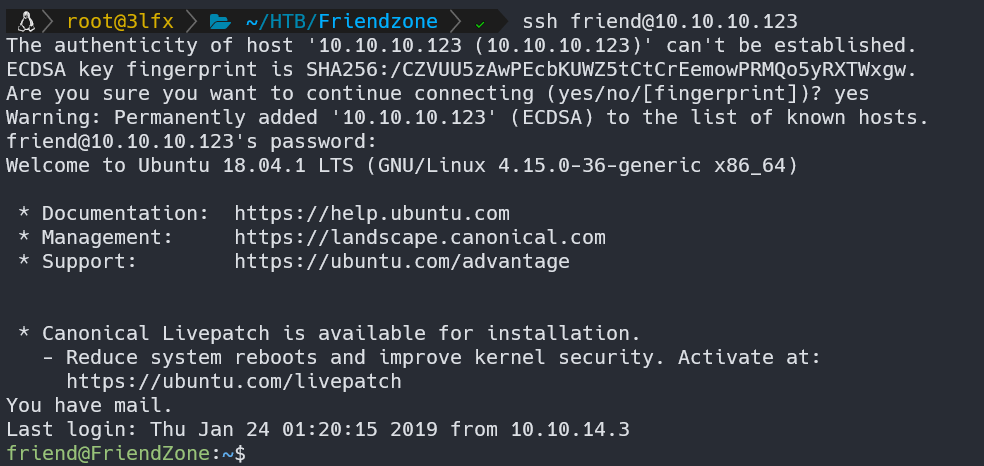
\includegraphics[width=0.99\textwidth]{informe4/imagenes/friendzone/22_conexionfriend.png}
            \caption{conexion en Friendzone} 
        \end{figure}

        \large{Nos ubicamos en la maquina y encontramos la flag.}
        \par
        \begin{figure}[H]
            \centering
            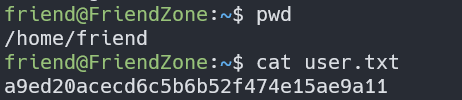
\includegraphics[width=0.99\textwidth]{informe4/imagenes/friendzone/23_1_flag_user.png}
            \caption{Flag user en Friendzone} 
        \end{figure}

        \large{Con la herramienta 'wget' subimos el 'linpeas.sh'.}
        \par
        \begin{figure}[H]
            \centering
            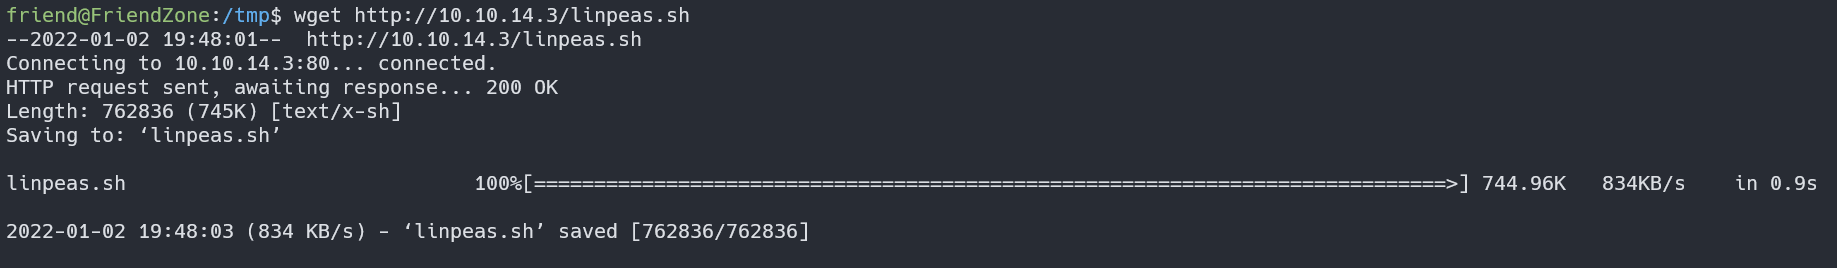
\includegraphics[width=0.99\textwidth]{informe4/imagenes/friendzone/23_2_uploadlinpeas.png}
            \caption{Upload linpeas en Friendzone} 
        \end{figure}

        \large{Buscamos credenciales en 'linpeas.sh'.}
        \par
        \begin{figure}[H]
            \centering
            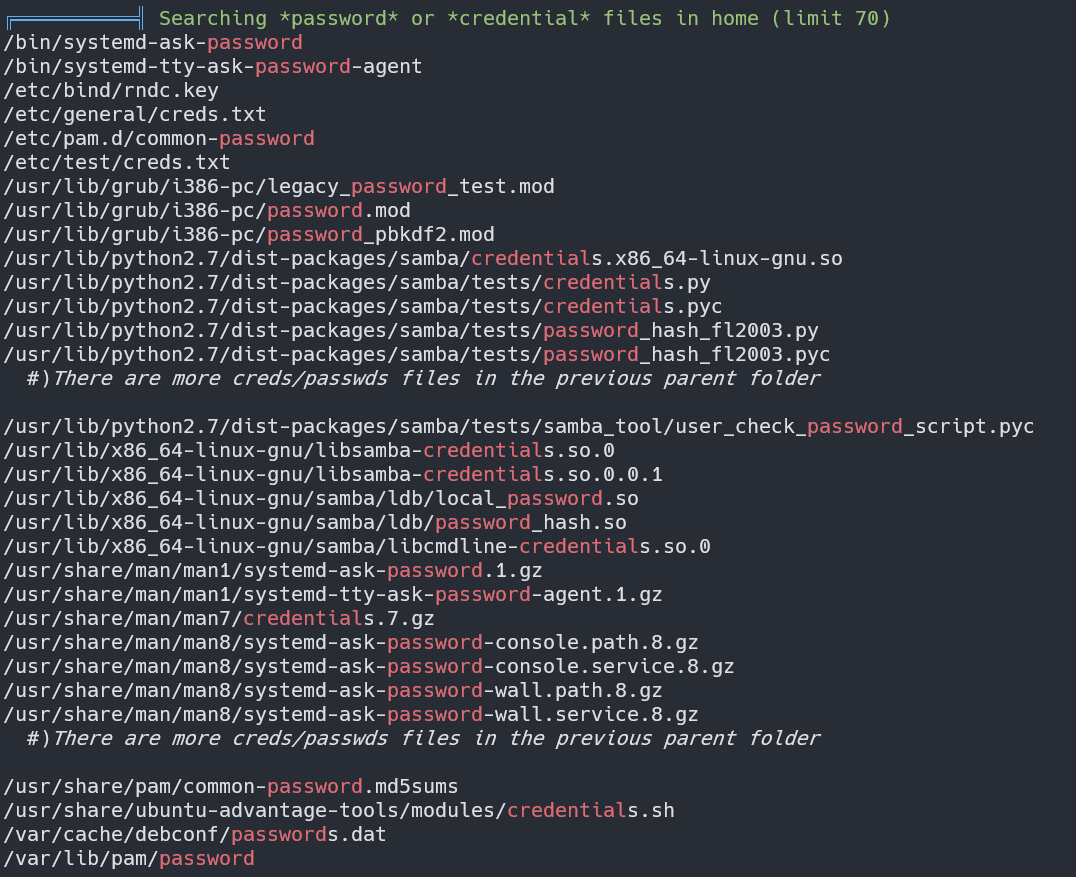
\includegraphics[width=0.99\textwidth]{informe4/imagenes/friendzone/24_linpeas.png}
            \caption{Linpeas en Friendzone} 
        \end{figure}


    \subsubsection{Post-Explotación}

    \subsubsection{Recomendaciones de Mitigación}

    
    \clearpage
%------Conclusiones-----------
\end{document}